\documentclass[letterpaper,11pt]{article}
\usepackage{myCV}

% bibliography
\usepackage{natbib}
\usepackage{bibentry}

% meta data
\name{Qilong Liu}
\email{qi-long.liu@connect.polyu.hk}

\addlink
    {https://scholar.google.com/citations?user=N2-7ArsAAAAJ&hl=en}
    {Google Scholar 
\includegraphics[height=0.3cm]{icon/google-scholar.png}}
\addlink
    {https://orcid.org/0000-0001-7843-1925}
    {ORCID 
\includegraphics[height=0.3cm]{icon/orcid.png}}
\addlink
    {https://github.com/liu-qilong}
    {GitHub 
\includegraphics[height=0.3cm]{icon/github.png}}
\addlink
    {https://liu-qilong.github.io}
    {Homepage 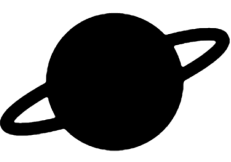
\includegraphics[height=0.3cm]{icon/blog.png}}

\begin{document}
    \maketitle

    % research interests
    \section{Research interests}

    \begin{resumeItemize}
        \item 3D vision; 4D spatial-temporal learning; AI4Design; Multi-agent.
    \end{resumeItemize}
    
    % education
    \section{Education}

    \resumeColumnsStart
        \resumeEntry
            {The Hong Kong Polytechnic University}{Jan 2025 -- }
            {Doctor of Philosophy, \href{https://www.polyu.edu.hk/sft/}{School of Fashion and Textiles}}{Hong Kong, China}
            \resumeSubline{and \href{https://www.aidlab.hk/en/}{Laboratory for Artificial Intelligence in Design (AiDLab)}}{}
            \resumeSubline{Supervised by \href{https://research.polyu.edu.hk/en/persons/kit-lun-yick}{Prof. Kit-lun Yick}}
        \resumeEntry
            {The Hong Kong Polytechnic University}{Sep 2021 -- Feb 2024}
            {Master of Philosophy, \href{https://www.polyu.edu.hk/sft/}{School of Fashion and Textiles}}{Hong Kong, China}
            \resumeSubline{and \href{https://www.aidlab.hk/en/}{Laboratory for Artificial Intelligence in Design (AiDLab)}}{}
            \resumeSubline{Supervised by \href{https://research.polyu.edu.hk/en/persons/kit-lun-yick}{Prof. Kit-lun Yick} and co-supervised by \href{https://www.polyu.edu.hk/en/pri/people/pri-people/dr-yip-yiu-wan-joanne/}{Prof. Joanne Yip} and Dr. Yue Sun}
        \resumeEntry
            {Shenzhen University}{Sep 2017 -- Jul 2021}
            {Bachelor of Engineering, School of Biomedical Engineering
            \href{https://www.shanghairanking.com/rankings/gras/2023/RS0208}{\textsl{(ARWU \#24)}}}{Shenzhen, China}
            \resumeSubline{Supervised by \href{https://bme.szu.edu.cn/20161/0229/35.html}{Dr. Yongjin Zhou}}
    \resumeColumnsEnd

    % publications
    \section{Publications}

    \bibliographystyle{unsrt}
    \nobibliography{publications.bib}

    \begin{resumeItemize}
        % \item \textbf{In Submission}
        % \item \bibentry{QinfengXiao2024}
        
        % \item \textbf{Under Review}
        
        \item \textbf{Journal}
        \item \bibentry{PuilingLi2025} \paralink{https://jcr.clarivate.com/jcr-jp/journal-profile?journal=SCI\%20REP-UK&year=2023}{JCR Q1, IF 3.8}
        \item \bibentry{LiuQilong2024} \paralink{https://jcr.clarivate.com/jcr-jp/journal-profile?journal=PLOS\%20ONE&year=2023}{JCR Q1, IF 2.9}
        \item \bibentry{ZhangLiying2024} \paralink{https://jcr.clarivate.com/jcr-jp/journal-profile?journal=IEEE\%20ACCESS&year=2023}{JCR Q2, IF 3.4}
        \item \bibentry{ChenJiazhen2024} \paralink{https://jcr.clarivate.com/jcr-jp/journal-profile?journal=BIOMECH\%20MODEL\%20MECHAN&year=2023}{JCR Q2, IF 3.0}
        % \item \bibentry{ZhangLiying2023}
        % \item \bibentry{ShiQiuqiong2022}
        \item \bibentry{ChenXi2020} \paralink{http://qikan.cqvip.com/Qikan/Journal/AssessmentReport?kind=3&id=8339&from=Qikan_Journal_Summary}{PKU Core, IF 1.7}
        
        \item \textbf{Conference}
        \item \bibentry{LiuQilong2022}

        \item \textbf{Thesis}
        \item \bibentry{LiuQilong2024a}
     \end{resumeItemize}

    % awards
    \section{Awards}

    \resumeColumnsStart
        \resumeEntry
            {PolyU Research Postgraduate Scholarship (PRPgS)}{2025 -- }
            {The Hong Kong Polytechnic University}{}
        \resumeEntry
            {The Hong Kong Polytechnic University Research Studentship}{2021 -- 2023}
            {The Hong Kong Polytechnic University}{}
        \resumeEntry
            {Star of Double Innovations (Group Award)}{2021}
            {Third Prize, Shenzhen University}{}
        \resumeEntry
            {National College Students Biomedical Engineering Innovation Design Competition}{2019}
            {Third Prize}{}
        \resumeEntry
            {National College Students Electronic Design Competition}{2019}
            {Third Prize in Guangdong Province}{}
    \resumeColumnsEnd

    % work experience
    \section{Work \& research experience}

    \resumeColumnsStart
        \resumeEntry
            {The Hong Kong Polytechnic University}{Sep 2023 -- Dec 2024}
            {Research Assistant (full-time)}{Hong Kong, China}
            \resumeSubline{Supervised by \href{https://research.polyu.edu.hk/en/persons/kit-lun-yick}{Prof. Kit-lun Yick}}
            \resumeSubline{3D/4D scene reconstruction/understanding, dense motion tracking, and human pose analysis}
        \resumeEntry
            {Shenzhen Base of The Hong Kong Polytechnic University}{Dec 2020 -- Jun 2021}
            {Student Assistant (part-time) for \href{https://research.polyu.edu.hk/en/persons/kit-lun-yick}{Prof. Kit-lun Yick}}{Shenzhen, Guangdong, China}
            \resumeSubline{Supervised by \href{https://research.polyu.edu.hk/en/persons/kit-lun-yick}{Prof. Kit-lun Yick}}
            \resumeSubline{3D/4D scanning data cleansing, labelling, and processing}
        \resumeEntry
            {Shenzhen Zhishixinyun Educational Technology Ltd.}{Nov 2019 -- Mar 2020}
            {Cofounder and Python tutorial lecturer}{Shenzhen, Guangdong, China}
            \resumeSubline{A campus startup that aims at providing short-term STEM and arts tutorials for college students}
    \resumeColumnsEnd

    % projects
    \section{Open-source projects \emph{(selected)}}

    \resumeColumnsStart
        \resumeEntry
            {BibTeX Scholar}{2025}
            {A note-first BibTeX management software}{\paralink{https://github.com/liu-qilong/mesh4d}{Link}}
        \resumeEntry
            {mesh4d}{2023}
            {Toolkit for 4D (3D + T) data visualisation, operation, and dynamic estimation}{\paralink{https://github.com/liu-qilong/bibtex-scholar}{Link}}
        \resumeEntry
            {PaperThread}{2023}
            {Visualize papers' relations as threads}{\paralink{https://github.com/liu-qilong/obsidian-setup}{Link}}
        \resumeEntry
            {FEcluster}{2023}
            {Distribute FE simulation tasks across multiple computers via SSH}{\paralink{https://github.com/liu-qilong/FEcluster}{Link}}
        \resumeEntry
            {Beamer-LaTeX-Themes}{2022}
            {Customized beamer templates for PolyU, SZU, and more}{\paralink{https://github.com/liu-qilong/Beamer-LaTeX-Themes}{Link}}
    \resumeColumnsEnd

    % skills
    \section{Skill set}

    \begin{resumeItemize}
        \item \textbf{Languages}. English (fluent); Mandarin (native); Cantonese (native)
        \item \textbf{Programming}. Python (seasoned); JavaScript \& Node.js \& CSS \& HTML (seasoned); LaTeX \& TikZ (seasoned).
    \end{resumeItemize}

\end{document}
